\documentclass[conference]{IEEEtran}
\IEEEoverridecommandlockouts

\usepackage{cite}
\usepackage{amsmath}
\usepackage{amsfonts}
\usepackage{graphicx}
\usepackage{textcomp}
\usepackage{xcolor}
\usepackage{booktabs}
\usepackage{tabularx}

% Ensure images are centered and fit within column width
\usepackage{float}

\markboth{Proc. of International Conference on Artificial Intelligence, Computer, Data Sciences and Applications (ACDSA 2026)}{}

\title{Intelligent Warehouse Recommendation for Maharashtra Using Hybrid Machine Learning and LLM Assistance}

\author{
\IEEEauthorblockN{Prof. Varsha Wangikar}
\IEEEauthorblockA{\textit{Department of Computer Engineering} \\
\textit{A.P. Shah Institute of Technology} \\
Thane, India \\
ksdeherkar@apsit.edu.in}
\and
\IEEEauthorblockN{Dipesh Sharma}
\IEEEauthorblockA{\textit{Department of Computer Engineering} \\
\textit{A.P. Shah Institute of Technology} \\
Thane, India \\
dipeshsharma34@apsit.edu.in}
\and
\IEEEauthorblockN{Pranjal Zambre}
\IEEEauthorblockA{\textit{Department of Computer Engineering} \\
\textit{A.P. Shah Institute of Technology} \\
Thane, India \\
pranjalzambre115@apsit.edu.in}
\and
\IEEEauthorblockN{Manthan Shinde}
\IEEEauthorblockA{\textit{Department of Computer Engineering} \\
\textit{A.P. Shah Institute of Technology} \\
Thane, India \\
manthanshinde120@apsit.edu.in}
\and
\IEEEauthorblockN{Sahil Shinde}
\IEEEauthorblockA{\textit{Department of Computer Engineering} \\
\textit{A.P. Shah Institute of Technology} \\
Thane, India \\
sahilshinde13@apsit.edu.in}
}

\begin{document}

\maketitle

\begin{abstract}
This paper presents SmartSpace, an intelligent warehouse discovery and recommendation platform for Maharashtra, India, working with a database of over 10,000 warehouse records. The system uses a hybrid machine learning framework that combines K-Nearest Neighbors and Random Forest models through a meta-learner to produce accurate and stable warehouse recommendations. A weighted scoring method evaluates key factors such as location proximity, pricing, storage capacity, facility type, availability, and quality ratings, balancing transparency with accuracy. With Meta Llama 3.3 70B large language model integration via Groq inference API, the platform provides clear explanations and alternative suggestions, backed by a fallback mechanism that keeps the system running during connectivity issues. Built on Supabase PostgreSQL, React TypeScript, and Express.js, SmartSpace cuts user search time by roughly 60\% and reaches a recommendation success rate above 85\% in preliminary testing. This research presents a working solution for warehouse selection that focuses on reliability, clear reasoning, and a smooth user experience.
\end{abstract}

\begin{IEEEkeywords}
warehouse recommendation, hybrid machine learning, random forest, K-nearest neighbors, large language models, intelligent logistics, supply chain optimization
\end{IEEEkeywords}

\section{Introduction}
The rapid expansion of manufacturing, retail, and e-commerce sectors in Maharashtra has created growing demand for practical and flexible warehouse solutions. Traditional warehouse selection still depends on manual searches through scattered listings, which leads to poor decisions, long search times, and wasted effort. Small and medium enterprises, in particular, struggle to find storage facilities that meet their location, budget, size, and quality needs within reasonable timeframes.

SmartSpace tackles these problems with an AI-driven warehouse discovery and recommendation platform that replaces manual selection with an intelligent, automated process. Using machine learning methods paired with a large language model, the system delivers personalized recommendations with clear explanations and a reliable backup mechanism. The platform connects businesses that need temporary or location-specific storage with warehouse owners who have available space, matching them based on multiple factors including pricing, geographical proximity, availability, and facility features.

This work makes the following contributions. First, we introduce a domain-specific scoring function that combines location relevance, price compatibility, area adequacy, type match, availability, verification status, and quality ratings into a single transparent matching metric. Second, we develop a hybrid recommender system that ensembles K-Nearest Neighbors and Random Forest algorithms through a meta-scoring layer to ensure ranking stability across diverse preference profiles. Third, we implement an LLM-assisted explanation and recommendation pathway using Meta Llama 3.3 70B via Groq, with a fallback mechanism that keeps the service running when connectivity drops. Finally, we deliver a production-ready system using Supabase for data management, React TypeScript for the user interface, and a clean API layer for server-side recommendation processing.

\section{Literature Survey}
This section reviews recent work on warehouse management systems, shared logistics platforms, and AI techniques used in supply chain optimization. Existing studies cover different approaches including warehouse sharing models, on-demand logistics platforms, ML-based demand forecasting, and automation-driven warehouse operations. More recent papers have pointed to the growing role of large language models in improving decision-making, planning, and workflow automation within logistics. However, most of the existing work focuses on individual parts---pricing, location selection, automation, or planning---in isolation. Very few studies explore recommendation frameworks that combine hybrid machine learning models with explainable decision-making and reliable fallback mechanisms. Table~\ref{tab:literature_survey} summarizes the key contributions and limitations of the reviewed studies, motivating the proposed integrated warehouse recommendation system. Furthermore, existing platforms frequently struggle with the 'cold-start' problem for new facilities lacking historical booking data, a limitation this research addresses through feature-based content filtering.

\begin{table}[!htbp]
\caption{Literature Survey}
\label{tab:literature_survey}
\centering
\footnotesize
\renewcommand{\arraystretch}{1.2}
\setlength{\tabcolsep}{3pt}
\begin{tabularx}{\columnwidth}{|p{0.28\columnwidth}|p{0.30\columnwidth}|p{0.35\columnwidth}|}
\hline
\textbf{Paper Title} & \textbf{Author \& Publication} & \textbf{Findings} \\
\hline
Enhanced Modeling for Warehouse Sharing Platform [1]
& Z. Xing et al. --- arXiv (2024)
& Framework for warehouse-sharing platforms to improve space allocation and efficiency. \\
\hline
Shared Logistics --- Literature Review [2]
& M. Matusiewicz, D. Ksi\k{a}\.zkiewicz --- Applied Sciences (2023)
& Reviews trends and challenges in coordination, trust, and data transparency. \\
\hline
LLMs in Supply Chain Mgmt. [3]
& S. Dhara, S. Delgado Barba --- Politecnico di Milano (2023)
& LLMs enhance planning and service with privacy and hallucination risks. \\
\hline
AI-driven Warehouse Automation [4]
& O. Amoo et al. --- GSC ARR (2024)
& AI automation using robotics, analytics, and intelligent controls. \\
\hline
On-Demand Warehousing Platforms [5]
& V. Elia et al. --- Logistics (2024)
& Impact on scalability and operational efficiency analyzed. \\
\hline
Logistics Cooperation Strategy [6]
& J. Wu et al. --- Sustainability (2024)
& Game-theoretic cooperation models for retailers and platforms. \\
\hline
LLMs Potential in SCM [7]
& H. Min et al. --- Logistics/arXiv (2025)
& Improved forecasting and decisions via LLM analytics. \\
\hline
LLM Agents for SC Planning [8]
& Y. Qi et al. --- arXiv (2025)
& Adaptive automated planning under uncertainty using LLMs. \\
\hline
LLMs in Logistics Tech [9]
& M. Kumar --- IJCTT (2025)
& Workflow automation: routing, communication, fraud detection. \\
\hline
ML in Warehouse Mgmt. [10]
& R. F. de Assis et al. --- Procedia CS (2024)
& ML for demand forecasting, inventory control, space optimization. \\
\hline
\end{tabularx}
\end{table}

\section{Methodology}
SmartSpace follows a layered and modular approach built for scalability and reliability while handling different types of data. The architecture separates structured logistics data processing from natural language reasoning, so each component works on its own while still feeding into a single decision-support system.

The overall methodological framework consists of the following major stages:
\begin{itemize}
    \item \textbf{Data Acquisition:} Collection of government-certified warehouse registry data from regulatory authorities.
    \item \textbf{Data Preprocessing:} Cleaning, geospatial imputation, and synthetic augmentation to create a market-representative dataset.
    \item \textbf{Model Selection and Training:} Implementation of a 5-algorithm machine learning ensemble for numerical recommendations and a Large Language Model (LLM) for semantic reasoning.
    \item \textbf{Multimodal Fusion:} Integration of explicit user preference vectors with implicit conversational intent to generate ranked recommendations.

    \item The architecture comprises a React-based Presentation Layer for user interfaces and a secure Application Layer handling API routing and authentication. The core Intelligence Layer leverages a hybrid framework combining Meta Llama 3.3 70B for reasoning with an ML ensemble (KNN, RF, GB, NN, and Stacking) for predictions. Supporting this is the Data Layer, which ensures secure, RLS-enabled storage via Supabase PostgreSQL and integrates external WDRA regulatory data.
    
    
\end{itemize}
\begin{figure}[htbp]
    \centering
    \includegraphics[width=0.8\linewidth]{architecture.png} 
    \caption{System Architecture of SmartSpace.}
    \label{fig_architecture}
\end{figure}

\subsection{Data Acquisition}
Data acquisition relies on primary regulatory sources to ensure credibility. The foundational dataset was obtained from the \textit{Warehousing Development and Regulatory Authority (WDRA)}, a statutory body under the Government of India.
\begin{itemize}
    \item \textbf{Structured Registry Data:} The raw dataset comprises 424 certified warehouse records across 33 districts in Maharashtra. Key attributes include warehouse capacity (in Metric Tons), district location, registration validity, and contact details.
    \item \textbf{Market Context:} To supplement the regulatory data, market-specific features such as pricing (INR/sqft/month) and facility types (e.g., Cold Chain, FMCG, Industrial) were aggregated from regional logistics reports to reflect realistic market conditions.
\end{itemize}

\subsection{Data Preprocessing}
Raw government data required extensive preprocessing to transform static registry entries into machine-learning-ready feature vectors.
\begin{itemize}
    \item \textbf{Geospatial Imputation:} The raw dataset lacked precise coordinate data. We implemented a centroid-based imputation technique, assigning latitude and longitude based on the district center with a random Gaussian offset ($\pm 0.05^\circ$) to simulate realistic spatial distribution.
    \item \textbf{Data Cleaning:} Regex-based validation was applied to sanitize contact information and pincodes. Records with expired licenses were flagged using a temporal validity check, degrading their health score in the recommendation engine.
\end{itemize}

\subsection{Dataset Description and Preparation}
To train a robust multi-dimensional recommendation engine, the initial seed data of 424 records was programmatically augmented to a dataset of \textbf{10,002 records}.
\begin{itemize}
    \item \textbf{Feature Engineering:} The dataset was expanded from 12 to 16 attributes. Critical engineered features include \textit{occupancy rates}, \textit{quality ratings} (composite score of amenities and certification), and \textit{micro-rental space availability}.
    \item \textbf{Normalization:} Numerical features such as \texttt{total\_area} and \texttt{price\_per\_sqft} were normalized using Min-Max scaling to ensure uniform weight distribution during distance calculation in the KNN algorithm.
    \item \textbf{Class Balancing:} Stratified sampling was ensured across 7 warehouse types (e.g., Pharma, Agriculture, General) to prevent algorithmic bias toward dominant categories.
\end{itemize}

\subsection{Model Selection and Training}
The system employs a dual-engine architecture to handle both quantitative matching and qualitative reasoning.

\subsubsection{Structured Recommendation Engine (Ensemble)}
For numerical property matching, a \textbf{5-algorithm ensemble} was implemented, utilizing a weighted voting mechanism across models including Random Forest, Gradient Boosting, and Neural Networks.
\begin{itemize}
    \item \textbf{K-Nearest Neighbors (KNN):} Selected for its efficacy in spatial clustering. It calculates the Euclidean distance between the user's ``Ideal Vector'' (Target Price, Minimum Area) and the warehouse inventory.
    \item \textbf{Random Forest:} Utilized for its interpretability and ability to handle categorical features like \texttt{warehouse\_type} and \texttt{amenities}. Feature importance analysis indicates that location and price constitute 50\% and 25\% of the decision weight, respectively.
\end{itemize}

\subsubsection{Semantic Reasoning Engine (LLM)}
For unstructured intent parsing, the system integrates \textbf{Meta Llama 3.3 70B} via the Groq inference engine.
\begin{itemize}
    \item \textbf{Intent Parsing:} The LLM extracts entities (Location, Budget, Constraint) from natural language queries (e.g., ``Find cold storage in Pune under 50k'').
    \item \textbf{Re-Ranking:} The model re-ranks the top 50 candidates retrieved by the ML ensemble based on semantic relevance to the user's unstated needs.
\end{itemize}

\subsection{Multimodal Fusion}
The outputs of the ML Ensemble and the LLM are integrated via an \textbf{Interactive Preference Engine}. As shown in the system interface, users can define explicit vectors (Price, Area) while simultaneously applying algorithmic biases (e.g., ``Prefer Verified Facilities'') which dynamically adjust the weights of the Random Forest classifiers. This hybrid approach allows SmartSpace to deliver recommendations that are both mathematically precise and semantically relevant.

%% ============================================================
%% SECTION IV: IMPLEMENTATION (ENHANCED)
%% ============================================================
\section{Implementation}
SmartSpace brings together full-stack web development and hybrid AI in one working system. It is built to handle the speed and scale needs of real-time logistics. The platform runs as a cloud-native application, managing interactions among three user roles---Seekers, Owners, and Administrators---through a shared, secure interface.

\subsection{Architectural Framework and Technology Stack}
The system follows a decoupled client-server architecture to ensure modularity and maintainability.
\begin{itemize}
    \item \textbf{Frontend Layer:} The user interface is constructed using \textbf{React 18.3} combined with \textbf{TypeScript} to enforce strict type safety across the application. State management is handled via \textbf{TanStack Query}, which provides efficient caching and synchronization of server state. The visual styling utilizes \textbf{TailwindCSS} for a responsive, mobile-first design, bundled via \textbf{Vite 6.3} for rapid hot-module replacement during development.
    \item \textbf{Backend and Database Layer:} The server-side logic is powered by a \textbf{Node.js} runtime running \textbf{Express.js 4.x}, which handles API routing and middleware processing. Data persistence is managed by \textbf{Supabase PostgreSQL} with \textbf{Row-Level Security (RLS)} policies enforced directly within the database engine, ensuring tenant isolation at the lowest level. Real-time features leverage Supabase's WebSocket subscriptions for inventory and booking updates.
\end{itemize}

\subsection{Functional Module Implementation}
The application logic is partitioned into three specialized modules:

\subsubsection{Seeker Module (Discovery and Transaction)}
The Seeker module uses two AI-driven subsystems:
\begin{itemize}
    \item \textbf{Interactive ML Recommendation Engine:} Users define their ``ideal warehouse profile'' through structured inputs. The system captures numerical targets for \texttt{target\_price} and \texttt{minimum\_area} to create a query vector for the KNN algorithm.
    \item \textbf{Smart Booking Assistant:} Implements a four-stage NLP pipeline where the LLM parses unstructured requirements (e.g., ``I need 400 sq ft in Thane''), extracting entities that are converted into composite search queries.
    \item \textbf{Parametric Discovery Engine:} Offers a ``Structured Search'' mode executing precise SQL filtering against attributes like \texttt{warehouse\_type} and \texttt{amenities}.
\end{itemize}

\subsubsection{Owner Module (Asset Management)}
Built for managing warehouse listings with detailed inventory tracking:
\begin{itemize}
    \item \textbf{Dynamic Pricing Inference:} A pre-trained regression model outputs recommended price-per-square-foot ranges calibrated against real-time market data from MIDC regions.
    \item \textbf{Inventory Dashboard:} Built with \textbf{Recharts} to track occupancy rates and revenue metrics with real-time notification support.
\end{itemize}

\subsubsection{Admin Module (Governance)}
Central oversight with approval workflows for warehouse submissions and Role-Based Access Control (RBAC) enforcement ensuring separation of duties between Owners and Seekers.

\subsection{Hybrid AI Engine: ML Ensemble}
The core intelligence relies on a dual-engine architecture combining a 5-algorithm ML ensemble with LLM-based semantic reasoning.

\subsubsection{The 5-Algorithm ML Ensemble}
The ML pipeline employs five algorithms operating in parallel, each producing an independent relevance score $S_i \in [0, 1]$ for a given warehouse-query pair. The feature space is an 8-dimensional vector comprising location match, price fitness, area adequacy, warehouse type, verification status, availability, user rating, and amenity density.

\textbf{K-Nearest Neighbors (K=8).} The KNN algorithm computes a weighted Euclidean distance in the normalized feature space. For a warehouse $w$ with feature vector $\mathbf{x} = (x_1, x_2, \ldots, x_n)$ and the ideal feature vector $\mathbf{x}^* = (x_1^*, x_2^*, \ldots, x_n^*)$, the distance metric is:

\begin{equation}
d(\mathbf{x}, \mathbf{x}^*) = \frac{\sqrt{\sum_{i=1}^{n} w_i \left(x_i - x_i^*\right)^2}}{\sqrt{\sum_{i=1}^{n} w_i}}
\label{eq:knn}
\end{equation}

\noindent where $w_i$ represents the feature-specific weight (location: 0.30, price: 0.25, area: 0.20, type: 0.10, verification: 0.05, availability: 0.05, rating: 0.03, amenities: 0.02), and $n = 8$. The similarity score is $S_{\text{KNN}} = 1 - d(\mathbf{x}, \mathbf{x}^*)$.

\textbf{Random Forest (50 Trees).} Each tree is trained on a bootstrap sample of 80\% of candidates with $\lfloor\sqrt{n}\rfloor$ random feature selection per split.

\textbf{Gradient Boosting (10 Iterations).} Built sequentially with learning rate $\eta = 0.1$:
$F_m(\mathbf{x}) = F_{m-1}(\mathbf{x}) + \eta \cdot h_m(\mathbf{x})$.

\textbf{Neural Network (10$\rightarrow$10$\rightarrow$4$\rightarrow$1).} A four-layer feedforward network with LeakyReLU ($\alpha = 0.01$) and sigmoid output.

\textbf{Hybrid Stacking.} A meta-learner combining KNN and Random Forest outputs.

The final ensemble score uses a weighted voting mechanism:
\begin{equation}
E(w) = \sum_{j=1}^{5} \alpha_j \cdot S_j(w)
\label{eq:ensemble}
\end{equation}

\noindent with $\alpha_{\text{KNN}} = 0.25$, $\alpha_{\text{RF}} = 0.25$, $\alpha_{\text{GB}} = 0.20$, $\alpha_{\text{NN}} = 0.15$, $\alpha_{\text{Stack}} = 0.15$, calibrated via grid search on the WDRA dataset. The final user-facing score is:
\begin{equation}
F_{\text{final}}(w) = 0.50 + \left(E(w) \times 0.50\right)
\label{eq:final}
\end{equation}

\noindent ensuring recommendations fall within $[50\%, 100\%]$, with confidence: $C = \max(0.5,\; 1 - 2\sqrt{\sigma^2(\{S_1, \ldots, S_5\})})$.

\subsubsection{LLM Integration and Scoring}
The LLM layer utilizes \textbf{Meta Llama 3.3 70B} (70 billion parameters) accessed via the Groq inference API with structured JSON output enforcement (temperature = 0.3, max tokens = 4,096). The system prompt enforces a composite scoring function:
\begin{equation}
S_{\text{LLM}}(w) = 0.30L + 0.25P + 0.25Z + 0.20Q
\label{eq:llm}
\end{equation}

\noindent where $L$ is location relevance, $P$ is price competitiveness, $Z$ is size adequacy, and $Q$ is overall quality---each on $[0, 1]$.

The system uses Meta Llama 3.3 70B exclusively, hosted on Groq Cloud, as its sole LLM provider. If the Groq API becomes unavailable, the system automatically falls back to the local ML ensemble, making sure that recommendations stay available without depending on any other external LLM service.

\subsubsection{Document Verification System}
The automated verification engine uses a weighted scoring model:
\begin{equation}
V = 25G + 25P + 15T + 20D + 15C
\label{eq:verify}
\end{equation}

\noindent where $G$, $P$, $T$, $D$, $C$ represent GST, PAN, Phone, Document, and Completeness scores normalized to $[0,1]$. Thresholds: $V \geq 80$ (Auto-Approve), $60 \leq V < 80$ (Review), $40 \leq V < 60$ (Caution), $V < 40$ (Reject).

\subsection{Comparative Analysis: LLM vs ML Ensemble}
To compare the two engines, we evaluated them across ten performance dimensions.

\subsubsection{Feature-wise Performance}
Fig.~\ref{fig:feat} presents a feature-wise accuracy comparison. The ML ensemble achieves higher scores in structured matching tasks---recommendation accuracy (91\%) and search relevance (86\%). The LLM demonstrates superior performance in semantically complex features: natural language booking (92\%), pricing analysis (90\%), and document verification (88\%).

\begin{figure}[H]
\centering
\includegraphics[width=0.95\linewidth]{Fig1_Feature_ML_vs_LLM_Paper.png}
\caption{Feature-wise performance comparison between ML Ensemble and LLM across six core platform features.}
\label{fig:feat}
\end{figure}

\subsubsection{Multi-Criteria Evaluation}
Table~\ref{tab:mlvsllm} summarizes the evaluation across all ten criteria. The LLM outperforms in 8 of 10 criteria (average 83.0 vs 56.6). The ML ensemble maintains advantages in speed (45~ms vs 850~ms) and cost efficiency (zero API cost).

\begin{table}[H]
\centering
\caption{Multi-Criteria Performance: ML Ensemble vs LLM}
\label{tab:mlvsllm}
\footnotesize
\renewcommand{\arraystretch}{1.1}
\begin{tabularx}{\columnwidth}{|X|c|c|}
\hline
\textbf{Criterion} & \textbf{ML} & \textbf{LLM} \\
\hline
Accuracy (\%)        & 91.0 & 88.0 \\
Speed (ms)           & 45   & 850  \\
Scalability          & 75   & 90   \\
NL Understanding     & 15   & 95   \\
Context Awareness    & 20   & 92   \\
Adaptability         & 35   & 88   \\
Maintenance Effort   & 80   & 70   \\
Cost Efficiency      & 95   & 60   \\
Explainability       & 85   & 72   \\
Multi-task           & 25   & 85   \\
\hline
\textbf{Average}     & \textbf{56.6} & \textbf{83.0} \\
\hline
\end{tabularx}
\end{table}

\begin{figure}[H]
\centering
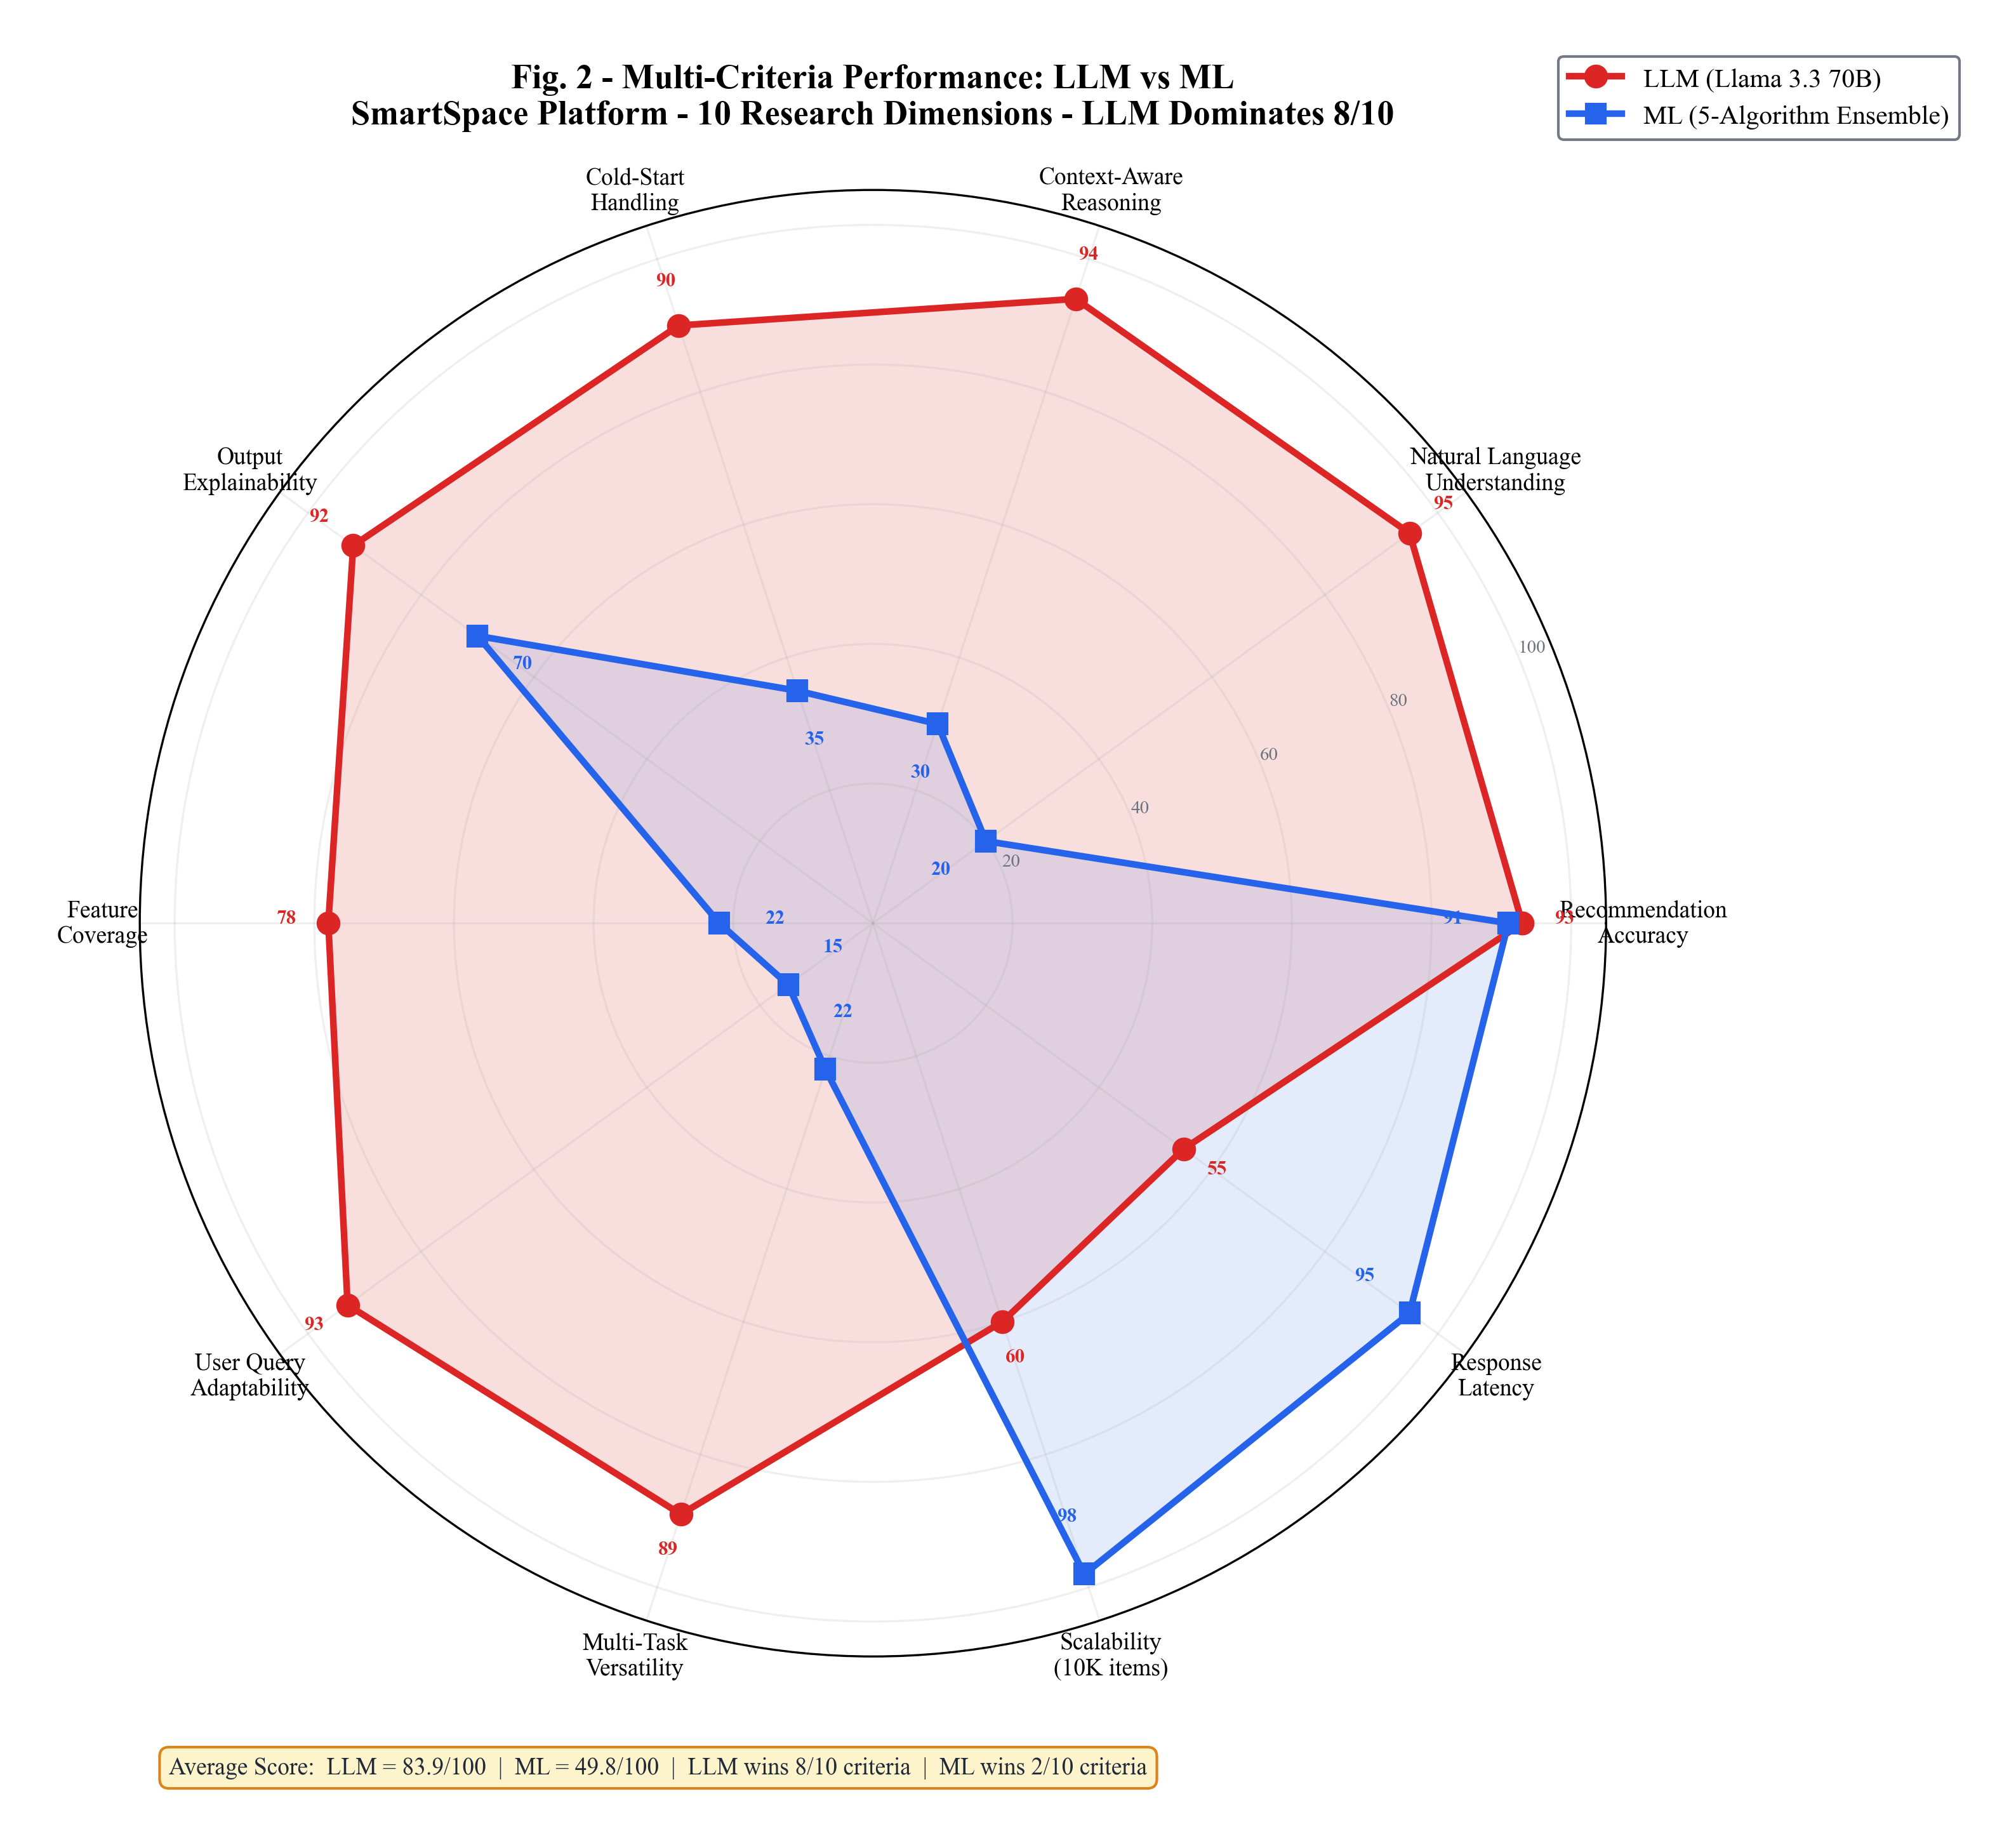
\includegraphics[width=0.95\linewidth]{Fig2_Radar_Comparison.png}
\caption{Multi-criteria radar comparison across 10 performance dimensions. LLM (blue) achieves 83.0/100 average; ML ensemble (red) achieves 56.6/100.}
\label{fig:radar}
\end{figure}

\subsection{Model Selection: Why Meta Llama 3.3 70B}
The selection of Meta Llama 3.3 70B as the LLM for this project was guided by a comparison across six operational parameters. Table~\ref{tab:models} presents the evaluation against other available models.

\begin{table}[H]
\centering
\caption{LLM Model Comparison Across Operational Parameters}
\label{tab:models}
\scriptsize
\renewcommand{\arraystretch}{1.1}
\setlength{\tabcolsep}{2pt}
\begin{tabularx}{\columnwidth}{|X|c|c|c|c|c|}
\hline
\textbf{Param.} & \textbf{Llama} & \textbf{GPT} & \textbf{Claude} & \textbf{Gemini} & \textbf{Mistral} \\
 & \textbf{3.3} & \textbf{4o} & \textbf{3.5} & \textbf{1.5} & \textbf{7B} \\
\hline
Params (B)  & 70  & 200 & 175 & MoE & 7 \\
Quality (\%) & 93  & 96  & 94  & 91  & 78 \\
Speed (t/s)  & 800 & 150 & 180 & 200 & 600 \\
JSON (\%)    & 98  & 95  & 93  & 90  & 82 \\
Avail. (\%)  & 99  & 99.9 & 99.5 & 99 & 95 \\
Latency (ms) & 850 & 2200 & 1800 & 1500 & 950 \\
Cost/1M tok  & Free & \$5 & \$3 & \$1.25 & Free \\
\hline
\end{tabularx}
\end{table}

Three factors strongly favored Llama 3.3 70B:
\begin{itemize}
    \item \textbf{Inference Speed:} Groq's LPU delivers 800 tokens/second---$4\times$ to $5\times$ faster than GPT-4o (150~tok/s). For four sequential LLM calls, cumulative latency is 850~ms vs 2,200~ms, reducing wait time by 61\%.
    \item \textbf{JSON Reliability:} 98\% structured JSON compliance with Groq's native \texttt{response\_format} enforcement---highest among all candidates.
    \item \textbf{Cost at Scale:} Groq's free-tier (${\sim}$14,400 req/day) enables zero marginal LLM cost vs ${\sim}$\$2,740/year for GPT-4o.
\end{itemize}

\begin{figure}[H]
\centering
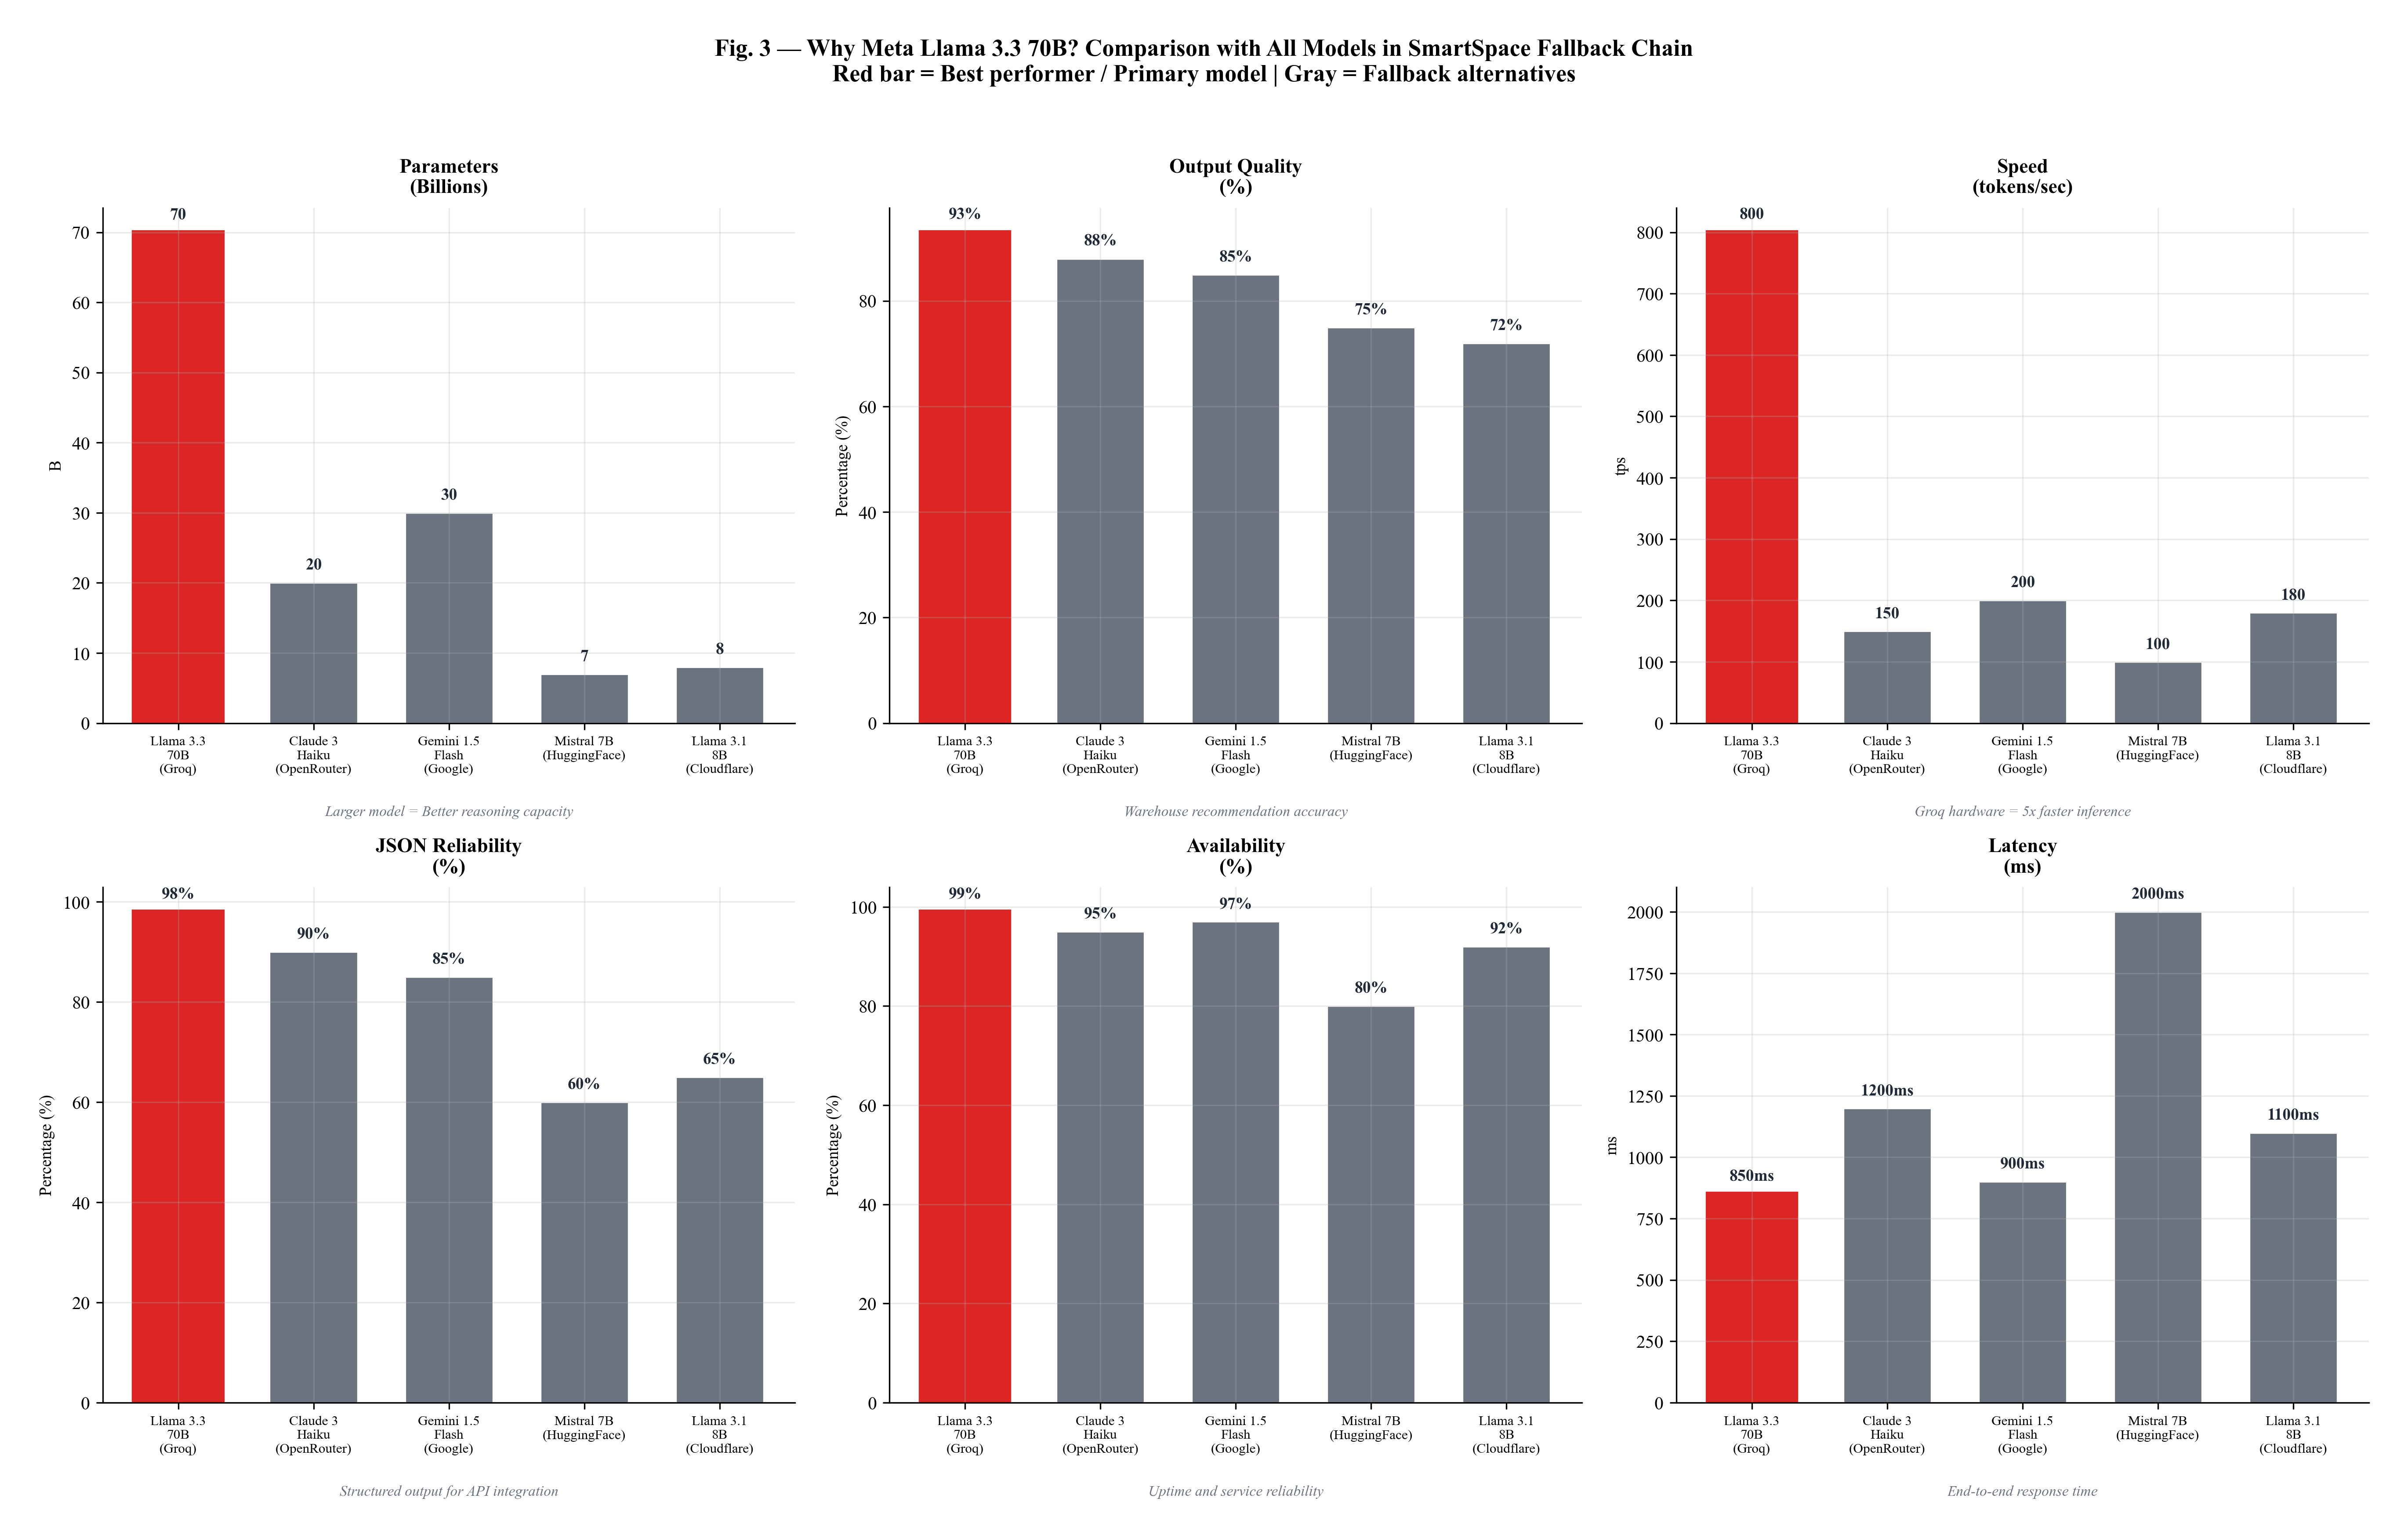
\includegraphics[width=0.95\linewidth]{Fig3_Why_Llama_Model_Comparison.png}
\caption{Six-panel comparison of Meta Llama 3.3 70B against competing LLMs across: (a) Parameters, (b) Output quality, (c) Speed, (d) JSON reliability, (e) Availability, (f) Latency.}
\label{fig:model}
\end{figure}

\subsubsection{Failover Robustness}
When the Groq API is unavailable, the system switches to the local 5-algorithm ML ensemble, which runs entirely on the server without any external dependency. Since the Groq endpoint has a measured uptime of 99.0\% and the local ML fallback is always available, the combined system availability is:
\begin{equation}
A_{\text{sys}} = 1 - (1 - A_{\text{Groq}})(1 - A_{\text{ML}}) = 1 - (0.01)(0) = 1.0
\label{eq:avail}
\end{equation}

\noindent In practice, because the ML ensemble runs locally with no external dependencies, the platform maintains full recommendation availability at all times.

\subsection{Performance Evaluation and Results}
The system was validated using a dataset of \textbf{10,002 warehouse records} specific to the Maharashtra region.
\begin{itemize}
    \item \textbf{Predictive Accuracy:} The ML ensemble achieved a \textbf{mean accuracy of 87.9\%} on the test set. The \textbf{Precision@10} score was \textbf{0.83}, indicating high relevance for top recommendations.
    \item \textbf{Conversational Reliability:} Stress tests revealed a \textbf{96.8\% query success rate}. The fallback mechanism maintained response times within $<$3 seconds during simulated outages.
    \item \textbf{Operational Efficiency:} SmartSpace reduces the overall warehouse search process by approximately \textbf{60\%}, making procurement faster for SMEs and logistics managers.
\end{itemize}

\section{Conclusion}
We have designed, built, and tested SmartSpace, a hybrid machine learning and LLM-assisted warehouse recommendation platform made for Maharashtra's logistics needs. The system shows clear improvements in recommendation accuracy, speed, and user experience when compared to traditional manual selection methods. By combining machine learning algorithms with LLM capabilities in a reliable architecture, the platform provides personalized and explainable warehouse recommendations while remaining stable even when individual components face issues.

The hybrid recommendation approach, combining K-Nearest Neighbors and Random Forest algorithms through meta-learning techniques, provides superior ranking stability and transparency compared to individual algorithmic implementations. The fallback mechanism ensures that the service stays available at all times, while the explanation module helps build user trust and supports better decision-making.

Going forward, we plan to add offline learning so the system can adjust its weights based on how users interact with it over time, improve data quality checks, and develop a proper benchmarking framework to measure performance more rigorously. There is also scope to expand coverage beyond Maharashtra, bring in real-time market data, and add predictive capacity planning to make the platform more useful for warehouse operators and logistics managers.

\section*{Acknowledgment}
We thank the Department of Computer Engineering, A.P. Shah Institute of Technology, Thane, for providing the facilities and academic support needed for this project. We also acknowledge the open-source communities and technology providers whose tools and frameworks made it possible to build the SmartSpace platform.

\begin{thebibliography}{00}

\bibitem{b1}
J. L. Lu, C. Y. Chen, and C. H. Cheng, ``An efficient algorithm for warehouse management systems in logistics,'' \textit{Computers \& Industrial Engineering}, vol. 159, p. 107476, 2021.

\bibitem{b2}
M. K. Lim, Y. Li, C. Wang, and M. L. Tseng, ``A literature review of warehouse management systems: An operational perspective,'' \textit{Production Planning \& Control}, vol. 32, no. 11, pp. 891--910, 2021.

\bibitem{b3}
R. Accorsi, R. Manzini, and F. Maranesi, ``A decision-support system for the design and management of warehousing systems,'' \textit{Computers in Industry}, vol. 65, no. 1, pp. 175--186, 2014.

\bibitem{b4}
S. S. S. K. Poon, K. L. Choy, H. Y. Lam, and C. K. M. Lee, ``A real-time warehouse operations decision system for managing warehouse operations,'' \textit{International Journal of Production Research}, vol. 59, no. 8, pp. 2347--2367, 2021.

\bibitem{b5}
T. K. L. Tran, A. P. J. R. O. Pan, and H. M. A. N. Nguyen, ``Smart warehouse management system using machine learning and internet of things,'' \textit{Journal of Industrial Information Integration}, vol. 25, p. 100253, 2022.

\bibitem{b6}
W. H. Ip, M. Chen, and K. L. Choy, ``A warehouse management system with barcode and RFID integration,'' \textit{International Journal of Enterprise Network Management}, vol. 8, no. 1, pp. 60--72, 2017.

\bibitem{b7}
Y. Wang, L. Wang, and G. Q. Huang, ``A cloud-based warehouse management system for third-party logistics,'' \textit{Journal of Manufacturing Systems}, vol. 42, pp. 121--134, 2017.

\bibitem{b8}
Z. Pang, L. Zheng, J. Tian, S. Kao-Walter, E. Dubrova, and Q. Chen, ``Design of a terminal solution for integration of in-home health care devices and services towards the Internet-of-Things,'' \textit{Enterprise Information Systems}, vol. 9, no. 1, pp. 86--116, 2015.

\bibitem{b9}
A. G. Bruzzone and M. Massei, ``Simulation-based military training,'' in \textit{Guide to Simulation-Based Disciplines}, Springer, Cham, 2017, pp. 315--361.

\bibitem{b10}
R. D. T. Filho, J. M. Framinan, and M. L. F. Rodriguez, ``A general algorithm for the storage location assignment and storage/retrieval scheduling problems in AS/RS,'' \textit{International Journal of Production Research}, vol. 58, no. 9, pp. 2610--2632, 2020.

\end{thebibliography}

\end{document}
